\documentclass[tikz]{standalone}
\usetikzlibrary{calc}
\usetikzlibrary{arrows.meta}

\usetikzlibrary{shapes.callouts}
\tikzset{
    gslevel/.style = {
        ultra thick,
        black,
    },
    eslevel/.style = {
        thick,
        black,
    },
    connect/.style = {
        dashed,
        black,
    },
    label/.style = {
        text width=2cm
    }
}
\begin{document}
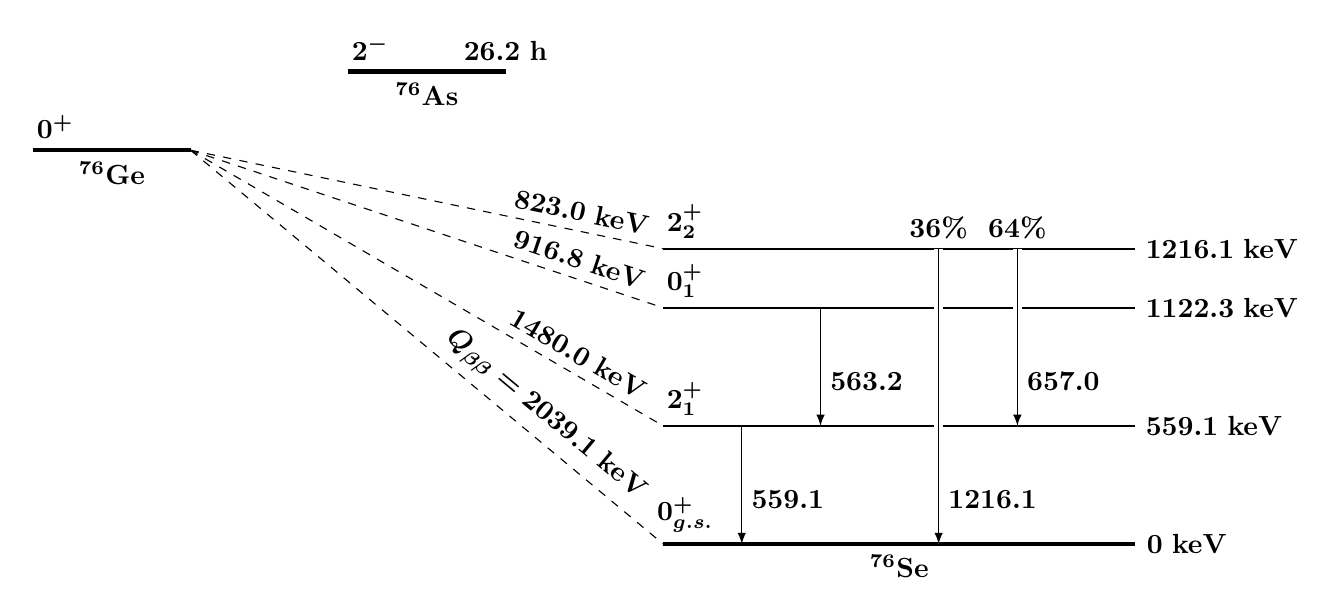
\begin{tikzpicture}[font=\boldmath]
  % Draw all levels

  \coordinate (GeLen) at (-2, 0);
  \coordinate (SeLen) at (6, 0);

  \coordinate (GeGS) at (2, 5);
  \coordinate (AsGS) at (4, 6);
  \coordinate (SeGS) at (8, 0);
  \coordinate (Se21) at (8, 1.5);
  \coordinate (Se01) at (8, 3);
  \coordinate (Se22) at (8, 3.75);
  
  \draw[gslevel] (GeGS) -- node[above, at end, xshift=8]{$0^+$} node[below] {$^{76}\mathrm{Ge}$} +(GeLen);
  \draw[gslevel] (AsGS) -- node[above, at start, xshift=8]{$2^-$} node[above, at end] {$26.2~\mathrm{h}$} node[below] {$^{76}\mathrm{As}$} +(2, 0);

  \draw[connect] (GeGS) edge node[sloped, above right, pos=0.5]{$Q_{\beta\beta}=2039.1~\mathrm{keV}$} (SeGS)
  (GeGS) edge node[sloped, above, pos=0.81]{$916.8~\mathrm{keV}$} (Se01)
  (GeGS) edge node[sloped, above, pos=0.8]{$1480.0~\mathrm{keV}$} (Se21)
  (GeGS) edge node[sloped, above, pos=0.82]{$823.0~\mathrm{keV}$} (Se22);
  
  \draw[eslevel] (Se22) -- node[above, at start, xshift=8] {$2^+_2$} node[at end, right] {$1216.1~\mathrm{keV}$} +(SeLen);
  \draw[eslevel] (Se01) -- node[above, at start, xshift=8] {$0^+_1$} node[at end, right] {$1122.3~\mathrm{keV}$} +(SeLen);
  \draw[eslevel] (Se21) -- node[above, at start, xshift=8] {$2^+_1$} node[at end, right] {$559.1~\mathrm{keV}$} +(SeLen);
  \draw[gslevel] (SeGS)     -- node[above, at start, xshift=8] {$0^+_{g.s.}$} node[at end, right] {$0~\mathrm{keV}$} node[below] {$^{76}\mathrm{Se}$} +(SeLen);

  \draw[-{latex[length=12pt]}] ($(Se21)+(1, 0)$)-- node[right, at end, yshift=16] {$559.1$}($(SeGS)+(1, 0)$);
  \draw[-{latex[length=12pt]}] ($(Se01)+(2, 0)$)-- node[right, at end, yshift=16] {$563.2$}($(Se21)+(2, 0)$);
  \draw[preaction={draw, line width=3pt, white}] [-{latex[length=12pt]}] ($(Se22)+(3.5, 0)$)-- node[right, at end, yshift=16] {$1216.1$} node[above, at start]{$36\%$} ($(SeGS)+(3.5, 0)$);
  \draw[preaction={draw, line width=3pt, white}] [-{latex[length=12pt]}] ($(Se22)+(4.5, 0)$)-- node[right, at end, yshift=16]{$657.0$} node[above, at start]{$64\%$} ($(Se21)+(4.5, 0)$);
  
\end{tikzpicture}
\end{document}